Op de donkere balk waarop ook Activities staat vind je aan de rechterkant een naar beneden wijzend driehoekje. Het
aanklikken van het driehoekje geeft een menu met daarop een overzicht van de helderheid van het scherm, aan welk
netwerk je gekoppeld bent, als je een laptop gebruikt wat de batterij status is, je loginnaam en drie knopjes die je
van links naar rechts toegang geven tot de systeemsettings, het locken van je scherm en het uitzetten of herstarten van
je machine.



\begin{figure}[H]
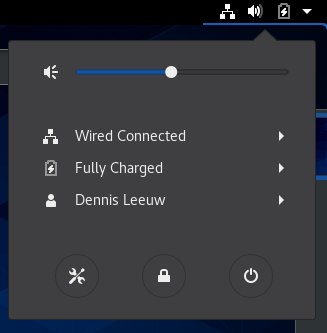
\includegraphics[width=0.9\textwidth]{linuxreader-img016.png}
\end{figure}
{\selectlanguage{dutch}
Selecteer Settings, scroll naar beneden naar Devices en selecteer deze, click dan op Displays. Trek het scherm los van
de topbar en schuif hem naar links. Click op de 800x600 resolutie en zet deze naar 1024x768}

{\selectlanguage{dutch}
\foreignlanguage{dutch}{Click op de Apply knop rechtsboven aan het scherm en daarna op Keep Settings. Natuurlijk mag je
resolutie ook hoger zetten, maar de minimale resolutie waarmee GNOME op CentOS 8 op een virtual machine prettig werkt
zonder dat je steeds met windows moet slepen is 1024x768. Selecteer {\textless} in de balk van Devices om terug te
komen in het hoofdmenu voor Settings. Loop door de verschillende opties om te ervaren waar je welke configuratie items
kan vinden en wijzigen.}}

\begin{figure}[H]
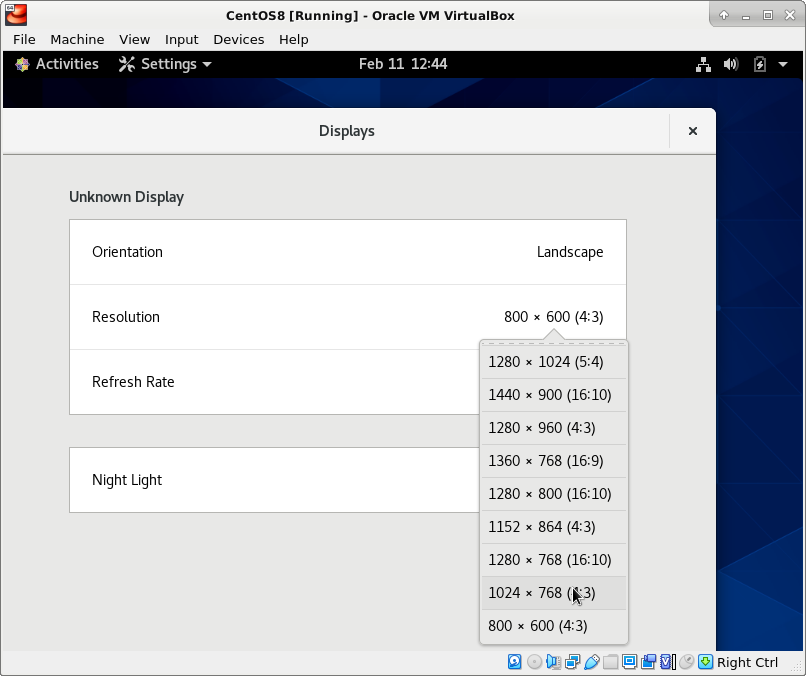
\includegraphics[width=0.9\textwidth]{linuxreader-img017.png}
\end{figure}
{\selectlanguage{dutch}
\foreignlanguage{dutch}{[TODO] Opdracht met documentatie in Writer om iets op te zoeken en te documenteren in Document1.
}}

